\chapter{Background}


Diffusion Tensor Imaging (DTI or DTMRI) is a recently developed Magnetic Resonance (MR) technique that provides information about the diffusion of water molecules in throughout the brain.  In white matter, due to the interactions between water molecules and the surrounding nerve fibers, the principle diffusion direction is aligned with the local fiber orientation.

White matter tractography is a visualization and analysis tool for DTI data.  It takes local diffusion information provided by DTI images and produces estimates of fiber bundles which may explain the observed global diffusion distribution.  White matter tractography provides a means of characterizing fiber bundles in-vivo and may provide insights into questions concerning white matter architecture.

A number of clinical studies have used tractography to compare fiber bundle characteristics in different populations.  Many of these studies utilize tractography methods which do not provide a measure of the confidence regarding the estimated fiber bundles.  The stochastic tractography system implemented in this research provides these measures of confidence, and may open new avenues of clinical investigation of white matter architecture.

\section{Neuroanatomy and Fiber Tracts}
\begin{figure} \label{fig:fibertracts}
	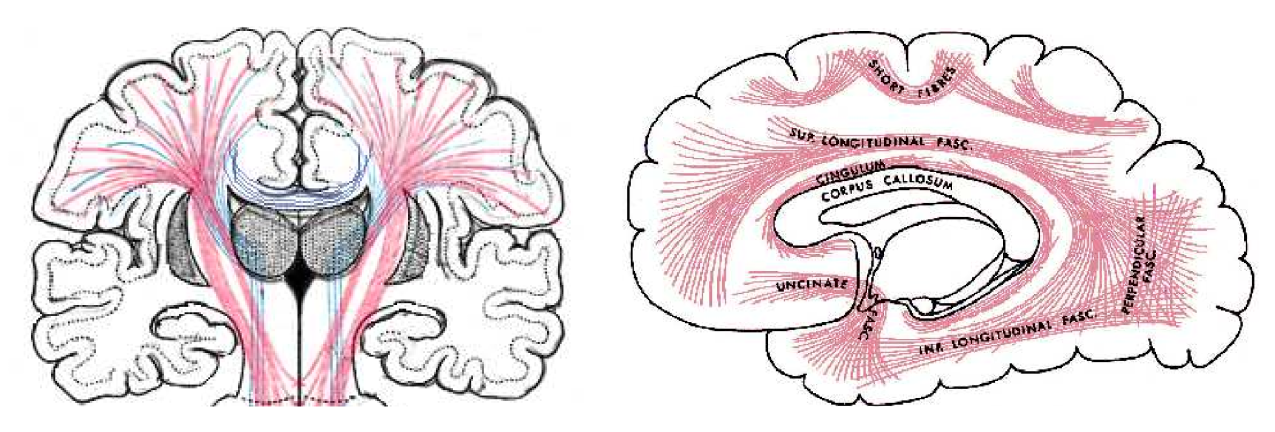
\includegraphics[width=\linewidth]{graysfibertracts}
	\caption{Example of human brain fiber tracts viewed from the front (coronal) and from the left (sagittal).  This image was derived from anatomical atlas diagrams in Gray's Anatomy \cite{odonnel06}.}
\end{figure}
Nerve tissue in the brain can be divided into gray and white matter.  Gray matter is found throughout the brain but is concentrated on the cortical surface as well as in structures deep within the brain such as the thalamus.  The defining characteristic of gray matter is its lack of myelinated axons.  In contrast white matter is white in color because it has an abundance of myelinated axons.  Myelin consists mostly of lipids and gives white matter its color.  Bundles of these axons comprise white matter tracts. Figure \ref{fig:fibertracts} illustrates some prominent fiber tracts.

\section{Diffusion Tensor MRI Physics}

Typically, MRI is used to differentiate between different tissue types, such as gray and white matter.  This technique works by magnetically polarizing a particular slice of the brain.  A strong uniform magnetic field is applied to the entire brain causing the spins of most of the electrons to orient in the same direction.  Another magnetic field, this one nonuniform in space, polarizes the spins of the atoms in the brain differently depending on their location.  This gradient field is turned off and as the spins of the electrons reorient, or relax, back to the strong uniform field, they release a radio signal which is picked up by the receiving coil.  The frequency of these waves depends on their polarization which is dependent on their position in space.  The time needed for the spins to relax, known as the relaxation time, depends on the type of tissue the molecules exist in.  Using this data, an image can be constructed that differentiates between tissue types due to their characteristic relaxation time. Unfortunately, white matter appears homogeneous in anatomical MRI images and do not provide much information about the orientation of the white fiber tracts within each voxel.  Without this information it is not possible to reliably determine the connectivity between different regions of gray matter.  Diffusion Tensor Imaging is a recently developed MR technique which provides more information to characterize fiber tracts.

Diffusion Tensor Imaging (DTI) or DTMRI is an imaging technique that indirectly provides information about fiber tract orientation from the diffusion profile of water in the brain tissues. Diffusion in many parts of the brain occurs anisotropically, meaning its rate of diffusion is directionally dependent.  This anisotropy is believed to be caused by local physical constraints that impede diffusion.  The diffusion of water molecules, which are the predominant signal emitters in MR imaging, is believed to be constrained by the myelin that surrounds axons.  DTI images describe the diffusion profile of water within each voxel using a diffusion tensor.  These tensors can be thought of as ellipsoids with the eigenvectors describing the major and minor axes of the ellipsoid and the associated eigenvalues scaling these axes.  Isotropic diffusion profiles result in spherical ellipsoids while anisotropic diffusion profiles produce more eccentric ellipsoids.  The parameters which describe these tensors are obtained from Diffusion Weighted Images (DWI) of the same volume captured using at least six unique gradient directions and one reference image obtained in the absence of weighting gradients.

Each Diffusion Weighted Image (DWI) provides information about the magnitude of diffusion in one particular direction.  Diffusion Weighted imaging works similarly to anatomical MRI imaging but is additionally able to capture the Brownian diffusion of molecules during the imaging process.  Unlike anatomical MRI, an additional gradient magnetic field is applied in a choosen direction which then makes the resulting observations sensitive to the self diffusion of water in that direction. An MRI image obtained using these diffusion sensitizing gradients is referred to as a Diffusion Weighted Image or DWI.  Associated with each of these images is the direction of the magnetic field gradient used to polarize the molecules.  This information is necessary because different magnetic field gradients may result in significantly different DWI images due to the anisotropy of diffusion in certain regions of the brain.  Finally, this diffusion information can be used to estimate the parameters of a diffusion tensor which is then used to infer the orientation of fiber tracts in that voxel.

\section{Diffusion Tensor}
The diffusion tensor is a 3x3 symetric matrix which describes the distribution of diffusion within each voxel.  Because the matrix is positive definite, its eigenvalues are positive and represent the magnetude of diffusion in the direction of the eigenvector associated with that eigenvalue.  The diffusion tensor is mostly represented as an ellipsoid, whose major and minor axis are described by the eigenvectors and associated eigenvalues of the tensor.  The eigenvector associated with the largest eigenvalue is sometimes referred to as the principle diffusion direction.  If the diffusion is sufficiently anisotropic, the principle diffusion direction is a good estimate of the local fiber orientation. %add physical meaning of the ellipsoid
%insert picture of ellipsoid

Because the tensor is sensitive to changes in the orientation of the object being scanned, clinical studies which attempt to compare different groups prefer to use properties of the tensor that are invariant to changes in orientation.  The most commonly used properties are the trace and the fractional anisotropy.  The trace the tensor is the sum of the diagonal components of the tensor and reprensents the average total diffusion.  A higher trace implies that there are few obstacles to water diffusion in that voxel.  The fraction anisotropy is given as
\begin{equation} \label{eq:tensormodel}
\sqrt{\frac{2*[(l\lambda_1-D_{av})^2 + (l\lambda_2-D_{av})^2 + (l\lambda_3-D_{av})^2]}
{2(\lambda_1^2+\lambda_2^2+\lambda_3^2)}}
\end{equation}

Fractional anisotropy is currently the most popular way to summarize the anisotropy of diffusion distribution expressed by the tensor.  FA ranges from 0 for isotropic diffusion to 1 for completely anisotropic diffusion.

%fill this in with related properties of the diffusion tensor
%various measures of anisotropy
%mathematic properties

\section{White Matter Tractography}

%[most have been voxel based,
% ROI studies, select a subset of voxels belonging to a particular fiber bundle of interest]
%[ROI studies sometimes select voxels in only one slice, which may not capture the information presented by the entire fiber tract...]


%[insert pictures]
%directionally coded images here
\begin{figure} \label{fig:visualization}
	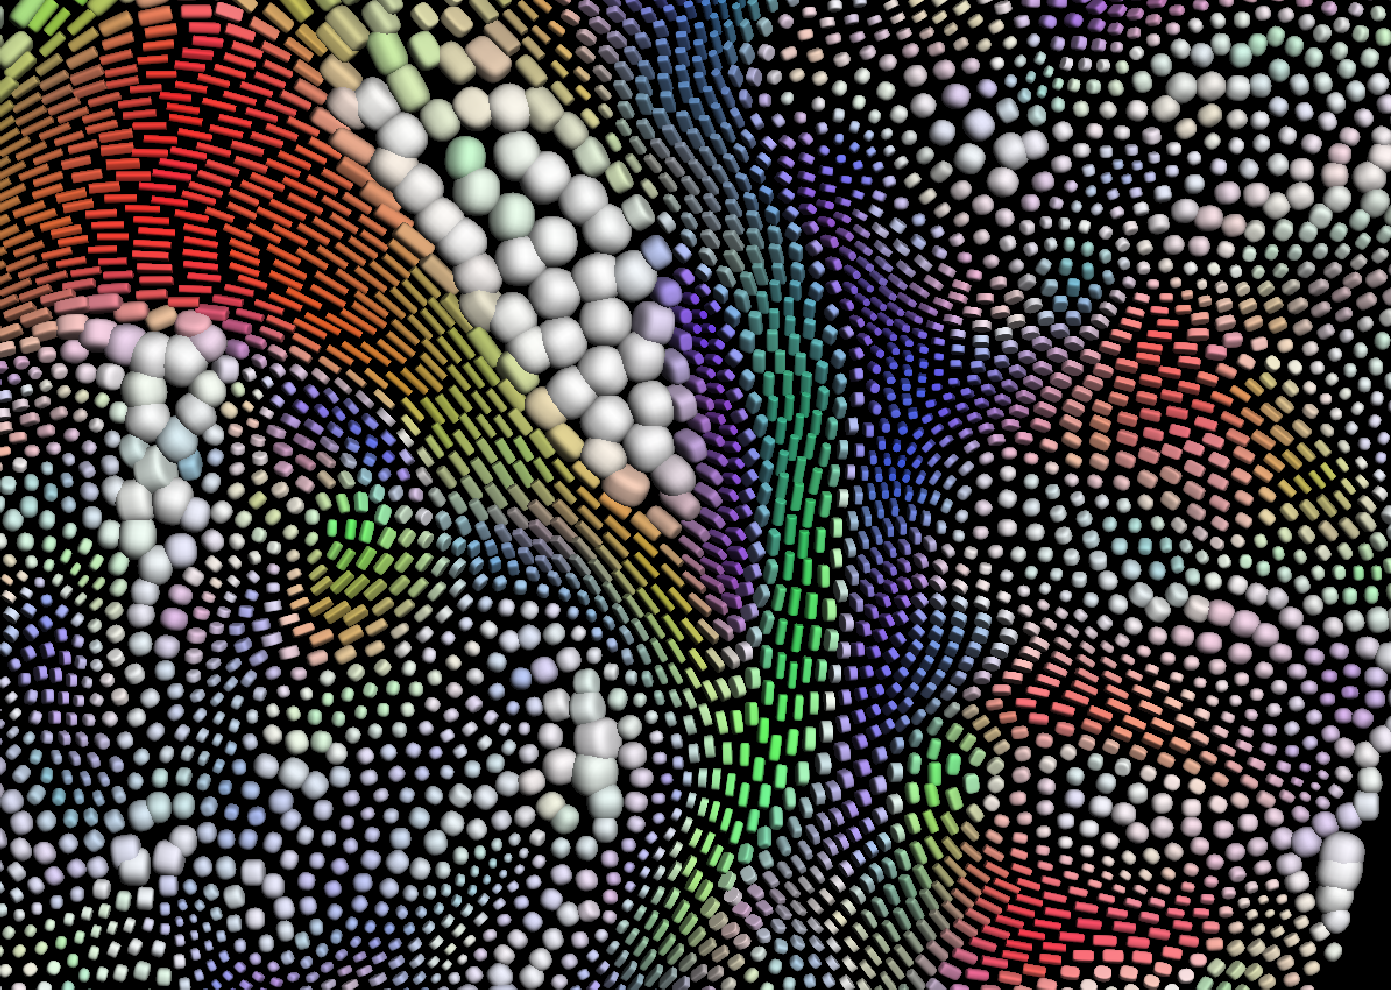
\includegraphics[width=0.5\linewidth]{packedglyphs}
	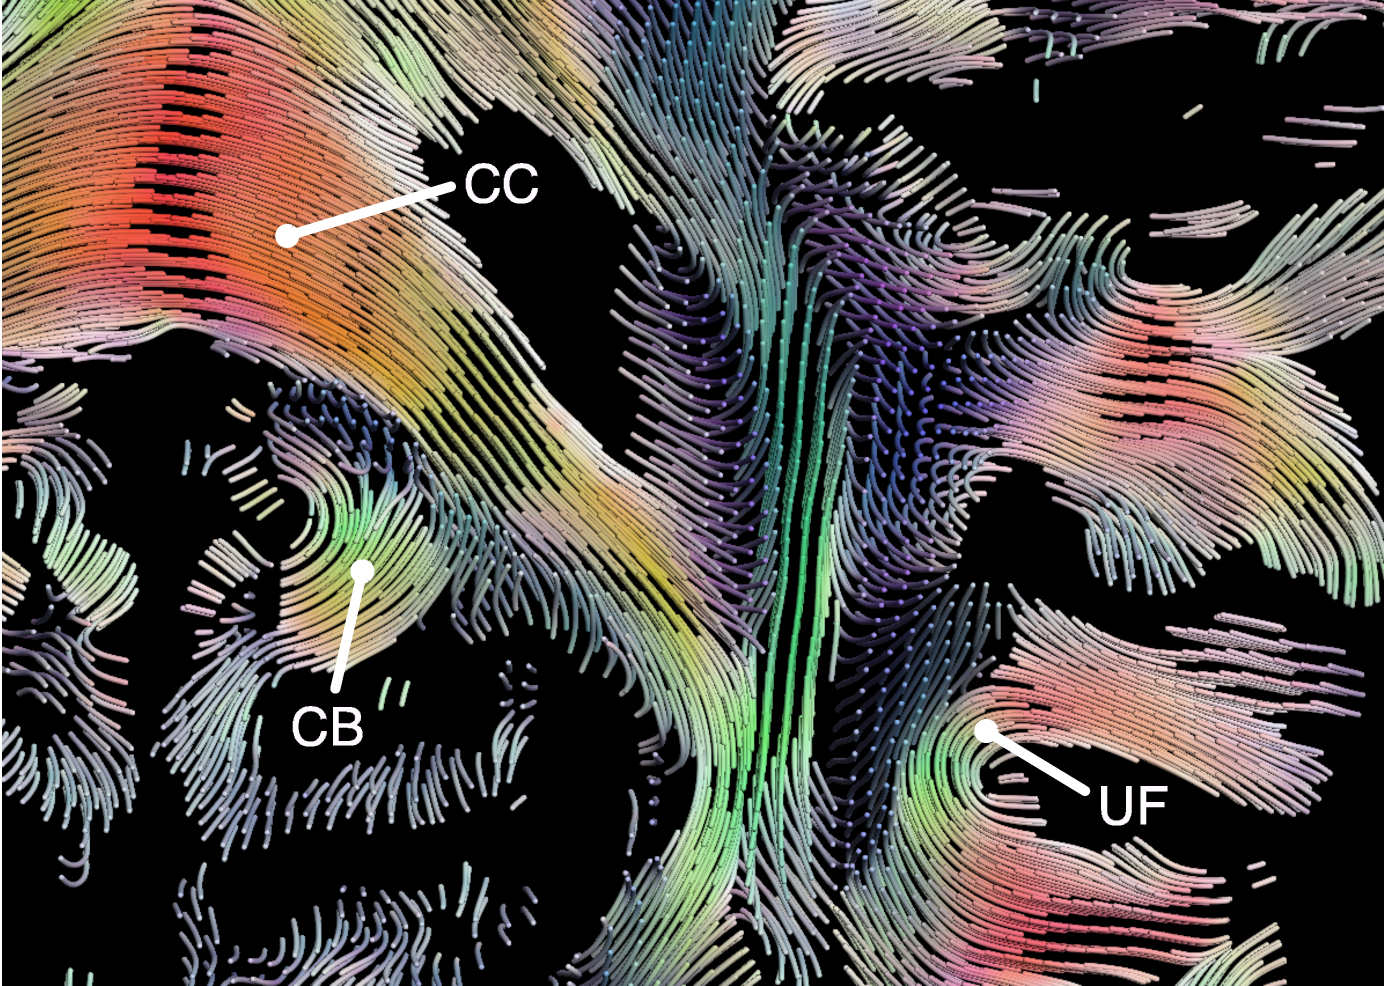
\includegraphics[width=0.5\linewidth]{tractography}
	\caption{DTI data visualization of major bundles using glyphs and streamlining tractography \cite{KindlmannTVCG2006}.  In the left image, DTI data is visualized using superquadric tensor glyphs. On the right, streamline tractography is performed on the same data.  The color in both images represent the estimated orientation of the fiber tract modulated by the degree of anisotropy in the data.  The color key is red is for left-right, blue for superior-inferior, green for anterior-posterior.  Regions that are white have low anisotropy while saturated regions exhibit highly anisotropic diffusion.}
\end{figure}


The two primary ways to visualize DTI data is through the use of glyphs and tractography.  Figure \ref{fig:visualization} demonstrates these two methods.  Glyphs are visual representations of the tensors at each voxel in one slice of DTI data.  The ellipsoid representation of the diffusion tensor can be also be used as a glyph but there exists many other representations that may provide a better visualization of the tensor field.  Glyph visualization is used for understanding diffusion in a localized region of interest.  Studies which compare local differences in DTI observations between different subjects are known as Region of Iterest or ROI studes. Although ROI analysis is straightforward, it is limited in the information it can provide and may actually introduce errors.  For instance, it is difficult to determine if observing a location along a fiber bundle in one patient corresponds to observing the same location in another patient.  Ultimately, clinical researchers are often interested in the global fiber bundles which produced these local DTI observations.  These fiber bundles span multiple voxels, limiting the usefulness of glyph visualization in holistic studies of fiber bundle characteristics.  These inquiries into the characteristics of fiber bundles led to the invention of white matter tractography.  In contrast with glyph visualization, white matter tractography incorporates diffusion information across multiple voxels in order to estimate a fiber bundle or bundles which could explain the observed diffusion data.

\subsection{Streamline Tractography Methods}
%talk about as many past works in DTI as possible
%name them by what the authors have called them
%Survey of White Matter Tractography
%Behrens
%Bootstrap
%Fast marching
%Stochastic Tractography

Tractography can be performed in a number of ways. One method is to draw tracts which are collinear with the principle direction of diffusion direction of every voxel it passes through.  These methods are collectively known as streamlining methods and have been suggested and characterized by a number of researchers \cite{behrensMRM03}.  Streamline tractography has relatively low computational cost and as such is very useful as a supplement to glyphs as a way to visualize DTI data.  However, streamline approaches do not provide information regarding the certainty of the estimated fiber tracts, limiting their usefulness in clinical studies which investigate white matter architecture characteristics.  Additionally, this lack of confidence information limits the regions that streamlining tractography can analyze.  Fiber orientation in regions which are highly isotropic are very uncertain.  Since streamlining methods do not account for this uncertainty, one cannot confidently analyze a region containing isotropic voxels using streamlining methods.  To reflect this limitation, many streamline methods will not estimate tracts which even momentarily pass through isotropic regions.  Unfortunately, isotropic voxels occur throughout the brain, even in regions with highly coherent fibers.  These voxels appear isotropic due to noise, distortions in the DTI data or due to limitations in imaging resolution which result in partial volume effects.  Partial volume effects are caused by fibers which cross within a single voxel.  Since these currently does not exist a widely accepted model to relate voxels containing multiple fiber orientations with the observed data, these crossings result in a diffusion distribution that is averaged amoung the crossing fiber, resulting in a diffusion distribution with reduced anisotropic.  Streamlining tractography's lack of robustness to isotropic diffusion limits its application in studies of fiber bundle characteristics.  These limitation motivated the invention of Stochastic or Probabilistic Tractography tractography algorithms.  This class of tractography algorithms overcomes the shortcomings of streamline methods by explicitly modeling the uncertainty in the local fiber orientation

\subsection{Stochastic Tractography Methods}
Stochastic tractography, sometimes known as probabilistic tractography, differs from streamlining methods in that it takes into account the uncertainty in fiber orientation when calculating estimates of fiber tracts.  Stochastic methods perform tractography under a probabilistic framework.  Under this framework, beliefs regarding the estimated local fiber orientation can be propagated to provide a measure of confidence regarding fiber tracts which span multiple voxels.  This explicit modeling and propagation of beliefs allows stochastic methods to generate tracts in regions of low anisotropy. Stochastic methods are able to generate tracts which momentarily pass through regions of low anisotropy because they integrate local fiber orientation uncertainty into the uncertainty of the entire tract.  The robustness of stochastic methods to local fiber orientation uncertainty has even enabled some studies to directly assess the connectivity of grey matter, which generally exhibits isotropic diffusion, with other regions of the brain\cite{behrensMRM03}.

\subsubsection{Bootstrap Method}

The Bootstrap Method is a stochastic method that calculates the degree of connectivity between different regions of the brain based on the variance in the original DTI data.  The obtains a measure of the variance of the DTI data by using redundant sets of DTI data and through the creation of new data which consist of recombinations of the original data.  In Jones et al. \cite{derek} research on the boot strap method, nine redundant sets of DWI volumes are obtained to perform the Bootstrap method.  Random combinations of portions of DWI volumes are sampled from this pool to generate a large number of complete mixed DWI sets known as bootstraps.  These complete mixed DWI sets are then converted to DTI images.  Standard streamline tractography is then performed on each bootstrap set at the same starting, or seed location.  A visitation percentage is then calculated for each voxel in the volume indicating the percentage of sample sets which generated a tract that passed through that particular voxel.  This visitation percentage can be interpreted as the probability that a voxel is connected to the seed point via a fiber tract.

\subsubsection{Bayesian Methods}
Stochastic tractography methods which use Bayesian frameworks express beliefs about estimated fiber tracts by generating a posterior probability distribution of fibers given the observed DTI data.   These tractography methods use a probabilistic model to relate the underlying fiber orientation with the observed DTI data.  The probabilistic model is applied to every voxel to generate a posterior distribution of possible fiber orientations given the observed diffusion in that voxel.  A streamline-like tractography method is then used to generate tracts by randomly sampling fiber directions from the fiber orientation posterior at each voxel as calculated by the local model.  The sampled tract is a realization of a random variable generated from the posterior distribution of fibers.  Since there are many possible paths, to obtain a good approximation of the posterior distribution of the, many paths must be sampled.  Additionally, similar to the Bootstrap method, the probability that region $A$ is connected to region $B$ can then be found by calculating the fraction of paths that pass through region $B$ originating from $A$.

Behrens's bayesian approach was one of the pioneering works in the field of stochastic tractography\cite{behrensMRM03}. An important idea in Behren's work is in keeping clear the distinction between estimating a general diffusion distribution from DWI data and estimating the local fiber orientation from DWI data.  Although an inference of the local fiber orientation can be made from the tensor model's principle diffusion direction, the tensor model is primarily a model to infer the distribution of diffusion given the data.  However, in stochastic tractography, we wish to infer the local fiber orientation from the observed diffusion data.  Behrens formulates this distinction by avoiding the tensor model altogether in favor of the two-compartment model. The two-compartment model makes the assumption that only a single fiber passes through a voxel.  Deviations from this simple model due to crossing fibers is captured as uncertainty in the fiber orientation.  In this model a voxel is described as two compartments whose net diffusion profile is the sum of a small anisotropic diffusion component that occurs in and around the fiber and a larger isotropic diffusion component outside of the fiber.\cite{behrensMRM03}.  The fiber orientation distribution is analytically intractable and Behrens overcomes this issue by computing the PDF using Markov Chain Monte Carlo (MCMC) techniques.  MCMC is a method to numerically integrate an analytically intractable integral.  
